\section{问题三的模型建立与求解}
\subsection{聚类分析确定打包方案}
问题三考虑到将位置较为集中的任务联合打包发布,从而提高了任务完成的
效率。因此,我们首先需要根据任务的位置信息判断哪些任务的位置分布较为集
中,从而确定打包方案。附件一给出的任务位置信息即为经纬度数据,首先,将
经纬度的数据作为地理位置的定量分析数据,利用聚类分析的方法,从位置分布
上对任务进行准确、细致的分类。此时,位置分布比较集中的任务会被自动归为
一类。我们将分析聚类结果的合理性,对于合理的分类,直接将此类中的任务联
合打包。对于不合理的分类,我们将对分类结果进一步调整后再打包。

Step 1:第一层聚类分析

首先,我们对聚类分析的分类数进行大致估算,由于任务总数为845 个,将
任务按照位置信息分为150 类时,平均每一类大约有5—6 个任务,这个数值比
较合理。因此,初次聚类时,将任务的位置分布分为150 类,利用Matlab 的
K-Means 命令得到的聚类分析图:

\begin{figure}[H]
    \centering
    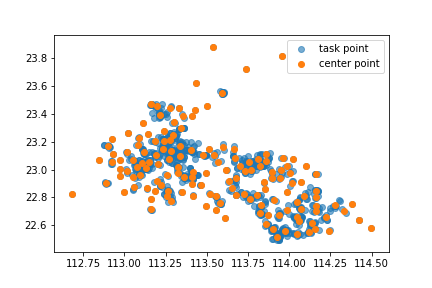
\includegraphics[width=1\textwidth]{150.png}
    \caption{K-Means聚类分析图}
    \label{}
\end{figure}

任务打包方案应当考虑两方面的问题:一是联合打包的任务应该在位置分布
上较为集中;二是一个任务包内的任务数量应当合理。我们假设一个任务包内的
任务数量取值范围为[2,15]。该聚类结果保证了一类中的任务在位置分布上较为
集中,下面来分析每个任务包中的任务数量是否符合假设。下图为每一类中任务
数量的统计图:
\begin{figure}[H]
    \centering
    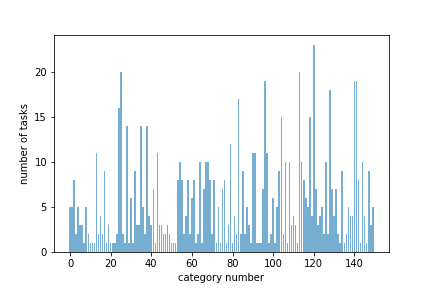
\includegraphics[width=1\textwidth]{tasks.png}
    \caption{每一类中任务数量的统计图}
    \label{}
\end{figure}

我们依据任务的位置信息将任务按照分布的集中度分成150 类,最多的类别
中有18 个任务。最少的类别中只有1 个任务。对于一类中只有1 个的任务,由
于其位置分布偏散,我们不对其做打包处理。但对于任务个数大于15 个的类别,
我们将这些任务位置信息提取出来,进行二次聚类分析。

Step 2:第二层聚类分析

我们假设当一类中任务数量不超过15 个时,这个打包方案才是合理的,在
上述聚类分析中,有九个类别中的任务数量超过了15 个.

对于这九个不合理的分类,我们在第一次分类结果的基础上,进行嵌套的聚
类分析,将它们分成两类。将这九个分类中的任务位置信息提取出来,再一次根
据其经纬度数据,利用Matlab 的K-Means 命令进行第二层聚类分析。
分别得到如下的分类图:

\begin{figure}
    \centering
    \begin{minipage}[c]{0.3\textwidth}
        \centering
        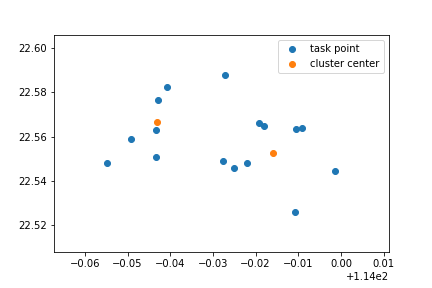
\includegraphics[width=0.95\textwidth]{24.png}
        \subcaption{第24类二次聚类图}
        \label{fig:sample-figure-a}
    \end{minipage}
    \begin{minipage}[c]{0.3\textwidth}
        \centering
        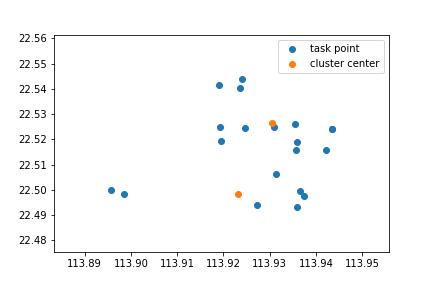
\includegraphics[width=0.95\textwidth]{25.png}
        \subcaption{第25类二次聚类图}
        \label{fig:sample-figure-b}
    \end{minipage}
    \begin{minipage}[c]{0.3\textwidth}
        \centering
        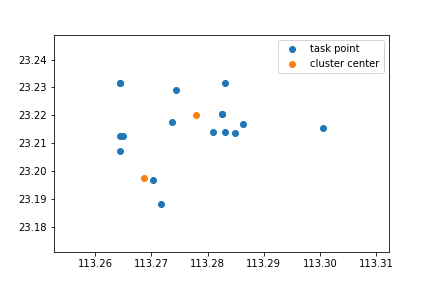
\includegraphics[width=0.95\textwidth]{83.png}
        \subcaption{第83类二次聚类图}
        \label{fig:sample-figure-c}
    \end{minipage}\\
    \begin{minipage}[c]{0.3\textwidth}
        \centering
        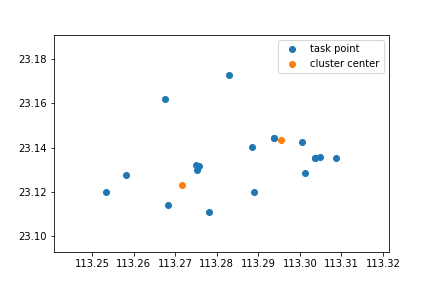
\includegraphics[width=0.95\textwidth]{96.png}
        \subcaption{第96类二次聚类图}
        \label{fig:sample-figure-a}
    \end{minipage}
    \begin{minipage}[c]{0.3\textwidth}
        \centering
        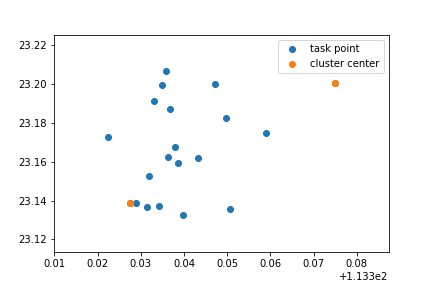
\includegraphics[width=0.95\textwidth]{113.png}
        \subcaption{第113类二次聚类图}
        \label{fig:sample-figure-b}
    \end{minipage}
    \begin{minipage}[c]{0.3\textwidth}
        \centering
        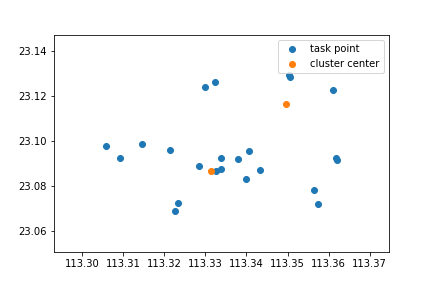
\includegraphics[width=0.95\textwidth]{120.png}
        \subcaption{第120类二次聚类图}
        \label{fig:sample-figure-c}
    \end{minipage}\\    \begin{minipage}[c]{0.3\textwidth}
        \centering
        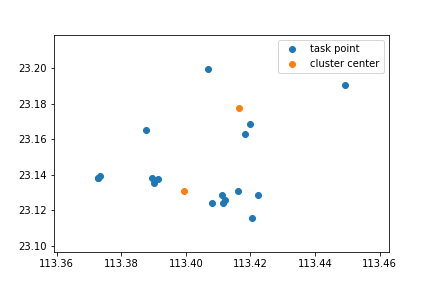
\includegraphics[width=0.95\textwidth]{128.png}
        \subcaption{第128类二次聚类图}
        \label{fig:sample-figure-a}
    \end{minipage}
    \begin{minipage}[c]{0.3\textwidth}
        \centering
        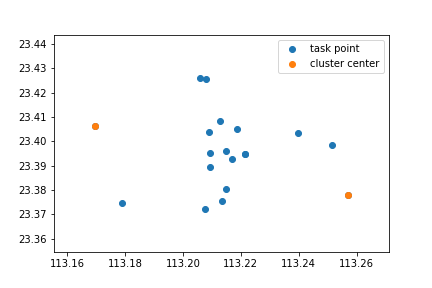
\includegraphics[width=0.95\textwidth]{140.png}
        \subcaption{第140类二次聚类图}
        \label{fig:sample-figure-b}
    \end{minipage}
    \begin{minipage}[c]{0.3\textwidth}
        \centering
        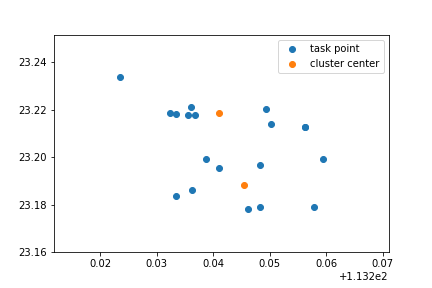
\includegraphics[width=0.95\textwidth]{141.png}
        \subcaption{第141类二次聚类图}
        \label{fig:sample-figure-c}
    \end{minipage}\\
    \caption{二重嵌套聚类分析图}
    \label{fig:sample-figure}
\end{figure}

对这九个类别进行嵌套聚类分析后,每一类别都由两个小类组成,每一小类
包含的任务数量由下面的统计表格给出:
% Please add the following required packages to your document preamble:
% \usepackage{multirow}
% \usepackage{longtable}
% Note: It may be necessary to compile the document several times to get a multi-page table to line up properly
\begin{longtable}[c]{ccc}
    \caption{嵌套聚类后任务数量}
    \label{tab:my-table}\\
    \hline
    类号                   & 新类别 & 再计数 \\ \hline
    \endfirsthead
    %
    \endhead
    %
    \multirow{2}{*}{24}  & 1   & 9   \\
                         & 2   & 7   \\ \hline
    \multirow{2}{*}{25}  & 1   & 7   \\
                         & 2   & 13  \\ \hline
    \multirow{2}{*}{83}  & 1   & 3   \\
                         & 2   & 14  \\ \hline
    \multirow{2}{*}{96}  & 1   & 8   \\
                         & 2   & 11  \\ \hline
    \multirow{2}{*}{113} & 1   & 12  \\
                         & 2   & 8   \\ \hline
    \multirow{2}{*}{120} & 1   & 7   \\
                         & 2   & 15  \\ \hline
    \multirow{2}{*}{128} & 1   & 5   \\
                         & 2   & 13  \\ \hline
    \multirow{2}{*}{140} & 1   & 12  \\
                         & 2   & 7   \\ \hline
    \multirow{2}{*}{141} & 1   & 10  \\
                         & 2   & 9   \\ \hline
    \end{longtable}
嵌套聚类分析后,每一类别的任务数量符合要求,此时得到的分类方案合理。


Step 3:确定任务打包方案

根据上述两次基于任务位置分布的聚类分析结果,我们将位置分布较为集中
的任务联合打包,同时保证每一个任务包内的任务数量不多于15 个,得到了一
个合理、准确的任务打包方案。

将一个任务包里的多个任务看做一个整体,与其它未被打包的任务同为一个
任务,经过联合打包处理过后的任务数量由835 个变为154 个。

\subsection{改进后的双目标定价优化模型}
利用聚类分析我们可以得到任务的打包方案,将位置分布较为集中的多个任
务进行联合打包,并将其看做一个整体,即为一个任务包,不论是没有打包的单
个任务还是一个任务包,我们在进行分析时都将其看做是一个任务。在问题二给
出的双目标优化定价模型中我们定义了一个吸引度矩阵,给出了矩阵中每一个元
素的计算公式,即:
$$w'_{i j}=\sqrt{\frac{0.01175}{l_{i j}^{2}}+0.000164 p_{i}^{2}}, \quad(\mathrm{i}=1,2 \cdots 835, \quad \mathrm{j}=1,2 \cdots 1875)$$
在对位置分布较为集中的多个任务进行打包处理后,任务总数会改变,需要
重新计算每个任务距离每位会员的距离,调整任务定价,从而吸引度矩阵的值会
发生相应变化。

经过聚类分析组合成的每个任务包都有一个中心点,我们将每个任务包的中
心点的经纬度坐标看作是这个任务的位置信息,计算每个任务包中心点与每位会
员之间距离。而对于那些位置分布较为松散,没有被打包处理的单个任务而言,
它们距离每位会员的距离不会发生改变。至此,我们得到打包处理后的距离矩阵
$L'_{ij}$,其中每个元素$l'_{ij}$表示任务$i $或者任务包$i $与会员$j $之间的距离。

经调整后的任务吸引度矩阵$W'_{ij}$中每个元素的表达式为:
$${w'}_{i j}^{\prime}=\sqrt{\frac{0.01175}{{l'}_{i j}^{\prime 2}}+0.000164 p_{i}^{2}}, \quad(\mathrm{i}=1,2 \cdots 154, \quad \mathrm{j}=1,2 \cdots 1875)$$

在利用双层嵌套聚类分析给出合理的打包方案后,任务总数变为154,这154
个任务预定过程依旧遵循问题二中的问题三是在对任务进行联合打包操作后,
对问题二的定价优化函数模型进行修改,在将多个位置比较集中的任务联合打包
发布的前提下,给出最优定价方案。因此,问题三实质上依旧是一个优化问题,
并且目标函数与问题二中模型的一致,通过改变约束条件来改变目标函数的求解
结果,从而修改前面的定价模型。得到在问题三的约束下的最优定价模型。

在修改后的优化模型中,发布的任务数量、距离矩阵、吸引度矩阵与
阈值均发生改变,建立起如下修改后的双目标定价优化模型:
$$\begin{aligned}
    & \begin{array}{l}
       \min \sum_{i=1}^{154} p_{i} \\
       \max \sum_{i=1}^{154} C_{i}
   \end{array} \\
    & s.t.\quad
   \begin{cases}
        & 50 \leq p_{i} \leq 100                                        \\
        & C_{i}=\left\{\begin{array}{ll}
           1, & w'_{i j}>w'_{i}      \\
           0, & w'_{i j} \leq w'_{i}
       \end{array}\right.                \\
        & {w'}_{i j}=\sqrt{\frac{0.01175}{{l'}_{i j}^{2}}+0.000164 p_{i}^{2}} \\
        & {w'}_{i}=\left\{\begin{array}{l}
           \min \left\{w'_{i j}\right\}, C_{i}=1 \\
           \max \left\{w'_{i j}\right\}, C_{i}=0
       \end{array}\right.                \\
        & \text {belong}(\mathrm{i})=j \mid \begin{array}{l}
           \max \left\{{w'}_{i j}\right\} \\
           \max \left\{G\left(n_{m}\right)\right\}
       \end{array}  \\
        & \begin{array}{ll}
           \text {choice1}(j)=i \mid & \begin{array}{l}
               \max \left\{{w'}_{i j}\right\}      \\
               \mathrm{i}=1,2 \cdots 154        \\
               j=1,2 \cdots, 7,14, \cdots, 1253 \\
               \text { belong }(\mathrm{i})
           \end{array}
       \end{array}                                    \\
       .                                                                \\
       .                                                                \\
       .                                                                \\
        & \begin{array}{l}
           \operatorname{choice} 31(j)=k\mid \begin{array}{l}
               \max \left\{{w'}_{i j}\right\} \\
               j=153,165,169, \cdots, 1875 \\
               \text { belong }(\mathrm{i})
           \end{array}
       \end{array}.
   \end{cases}
\end{aligned}
$$
\subsection{模型的求解}
\subsubsection{模型求解分析}
问题三的模型建立在问题二的模型之上,仍然考虑对模型中的约束进行一定
简化,并做出适当假设,得到全局最优解的近似解作为模型最优解。问题三模型
任务安排采用打包分配模式,首先通过聚类把类似的任务聚成一类,从而降低了
任务的维度。新的任务数即打包数量影响着任务阈值、吸引度矩阵等变量,通过
聚类打包求得新的任务情况,从而套用问题二的算法,对部分变量和维度进行修
改,经过遍历得到更优结果。
\subsubsection{模型求解步骤}
Step1:聚类打包

通过聚类算法,对任务进行分类,相似度较高的任务归为一类成为一个任务
包。部分个体未归入聚类类别的单独视为一个任务包。

Step2:预先设置任务定价

采用与问题二不同的定价模式。根据聚类,分别得到每个打包任务中单个任
务的最高、平均、最低价格,从而分为三种情况,分别将每个包中最高、平均、
最低作为打包任务的整体平均值。

Step3:吸引度矩阵更新

更新得到计算会员与每个打包之间的距离,并根据模型二,由吸引度计算公
式对每个任务对于每个会员的吸引度矩阵重新进行计算。

Step4:冲突判断

判断位置记录矩阵中,是否存在数值相等的情况,即判断是否存在冲突。若发生冲突,则对会员的信誉值进行比较,从而确定一个优先选择,即信誉高的会员得
到此次任务预定权。

Step5:方案及完成度结果

通过对时间和任务预定数的遍历,得到最终任务完成度矩阵,并输出任务完成度
数值,同时输出预先设定的任务定价矩阵。考虑到对复杂度和运行时间降低,不
采用对定价进行遍历的方式,而通过对任务定价矩阵的不同设置得到几组不同结
果,从而对比分析得到近似最优解。
\subsection{模型求解结果}
在对模型求解时,设定几组不同的价格调整比例,得到835 个任务的定价以
及任务完成度,由于结果数据庞大,此处只展示部分结果:
% Please add the following required packages to your document preamble:
% \usepackage{longtable}
% Note: It may be necessary to compile the document several times to get a multi-page table to line up properly
\begin{longtable}[c]{cccccc}
    \caption{}
    \label{tab:my-table}\\
    \hline
            & 每单定价 & 69.80 & 69.55 & 72.22 & 71.68 \\
    \endfirsthead
    %
    \endhead
    %
    \hline
    \endfoot
    %
    \endlastfoot
    %
    a=1.1   & 完成与否 & 1     & 0     & 1     & 1     \\
    b=0.99  & 成本   & \multicolumn{4}{c}{45,762}    \\
            & 完成率  & \multicolumn{4}{c}{0.76}      \\
            & 每单定价 & 70.15 & 69.90 & 72.22 & 71.68 \\
    a=1.1   & 完成与否 & 1     & 1     & 1     & 1     \\
    b=0.995 & 成本   & \multicolumn{4}{c}{52,403}    \\
            & 完成率  & \multicolumn{4}{c}{0.87}      \\
            & 每单定价 & 70.15 & 69.90 & 75.50 & 74.94 \\
    a=1.15  & 完成与否 & 1     & 1     & 1     & 1     \\
    b=0.995 & 成本   & \multicolumn{4}{c}{53,563}    \\
            & 完成率  & \multicolumn{4}{c}{0.87}      \\
            & 每单定价 & 69.80 & 69.55 & 75.50 & 74.84 \\
    a=1.15  & 完成与否 & 1     & 1     & 0     & 1     \\
    b=0.99  & 成本   & \multicolumn{4}{c}{46,921}    \\
            & 完成率  & \multicolumn{4}{c}{0.76}      \\ \hline
    \end{longtable}